
\begin{figure}
	\begin{center}
		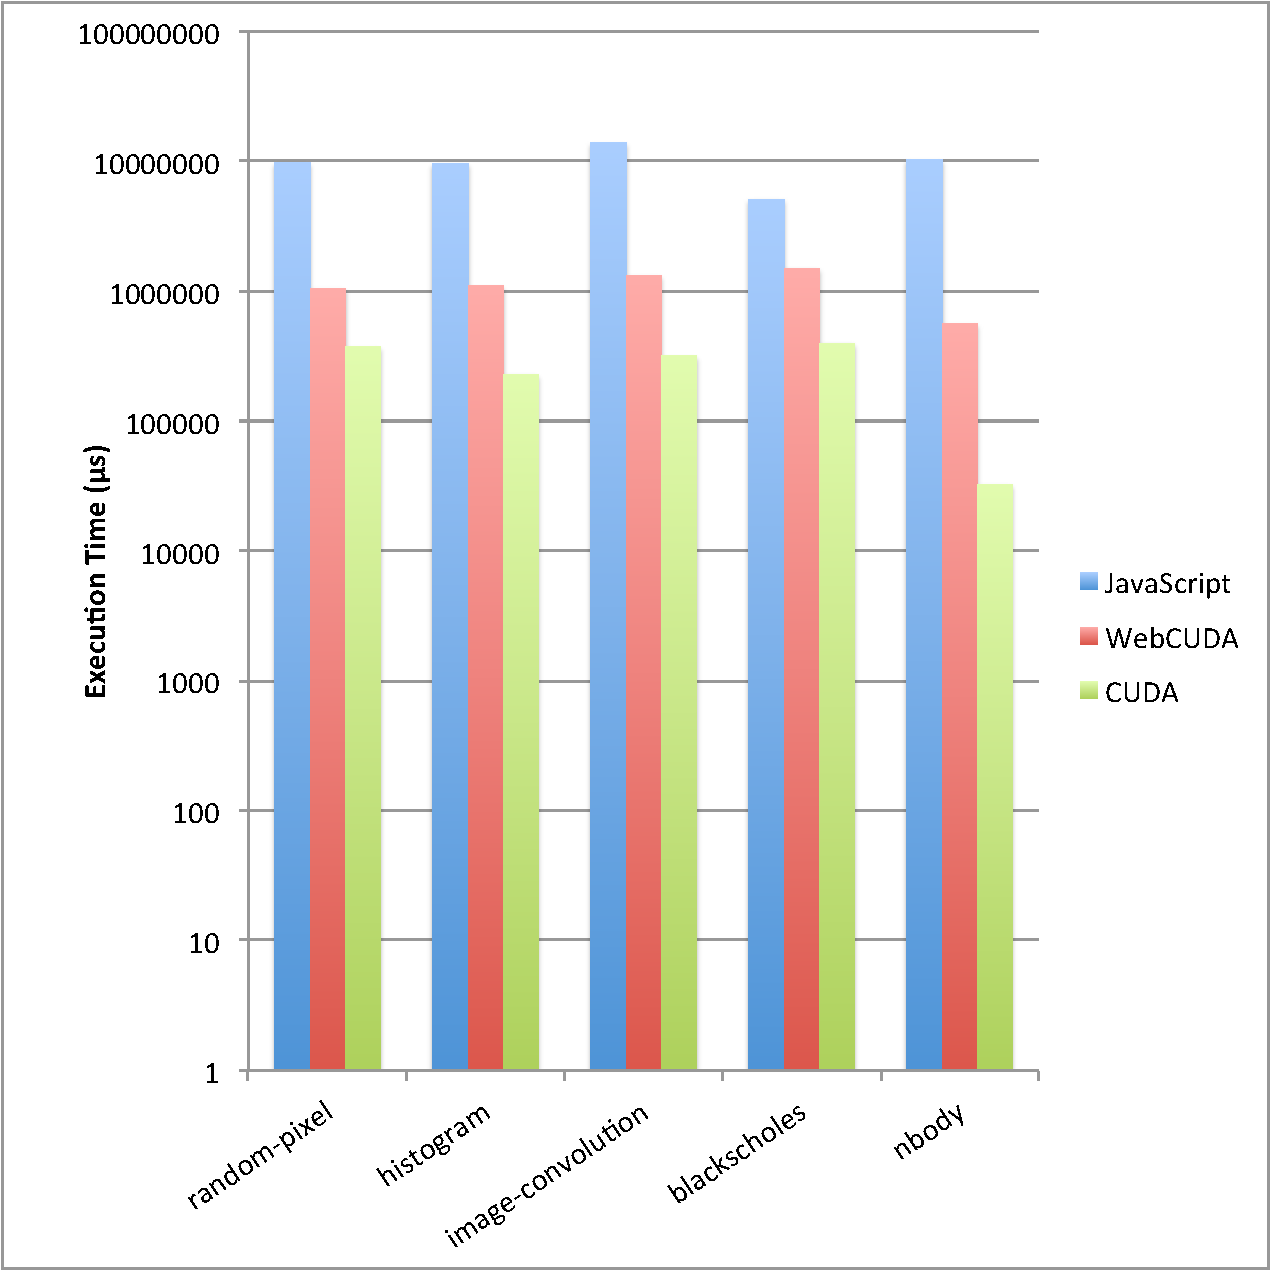
\includegraphics[width=\columnwidth]{./figures/fig1}
	\end{center}
	\caption{Creating new \name Device Object}
	\label{v8codea}
\end{figure}

\begin{figure}
	\begin{center}
		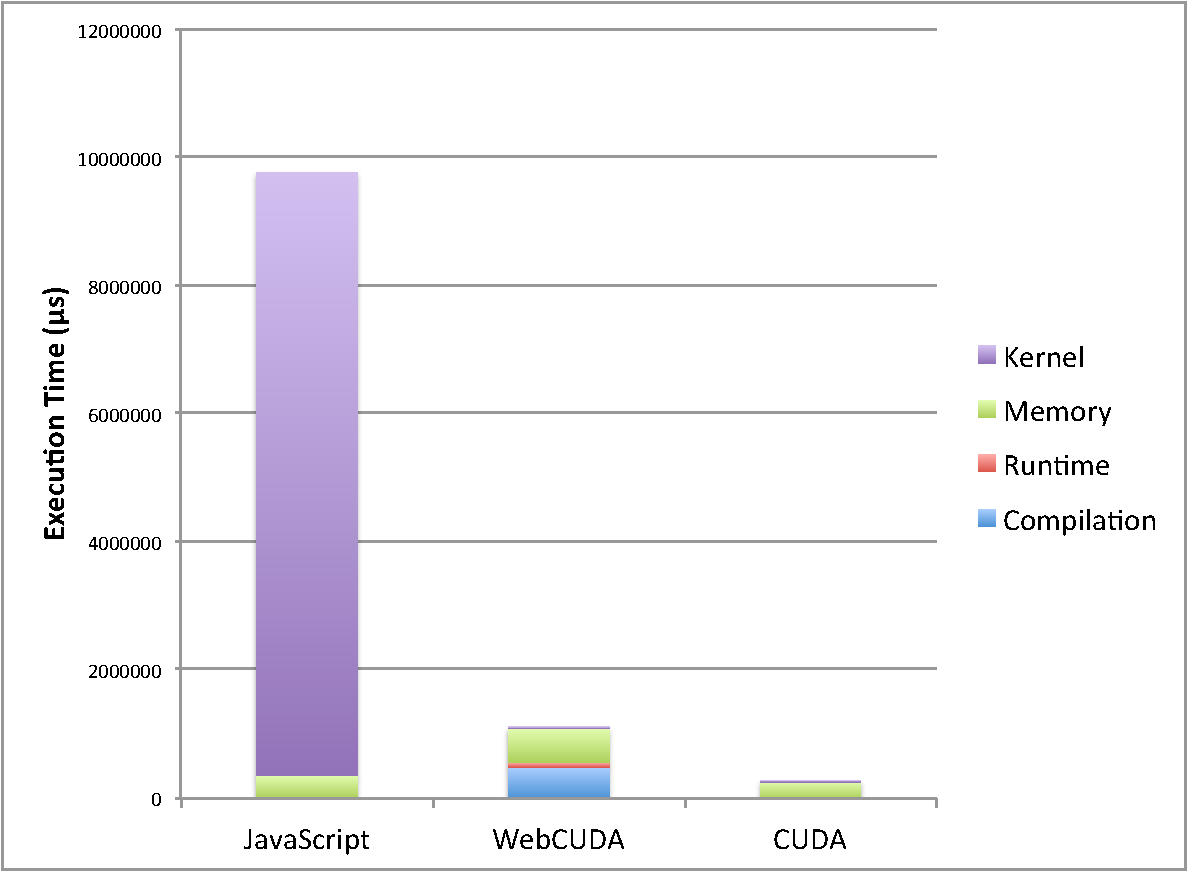
\includegraphics[width=\columnwidth]{./figures/fig2}
	\end{center}
	\caption{Creating new \name Device Object}
	\label{v8codea}
\end{figure}

\subsection{Benchmarks}
there should probably be a table here...
%TODO make table listing benchmarks, data sets
\begin{table}
	\begin{center}
		\begin{tabular}{| l | l |}
			\hline
			Benchname & Input Size \\
			\hline
			random-pixel & N/A \\
			\hline
			Nbody &  1024 bodies \\
			\hline
		\end{tabular}
	\end{center}
	\caption{Description of Benchmarks use for evaluation.}
	\label{benchmark-table}
\end{table}

\paragraph{Random Pixel Generator}

\paragraph{N-Body Force Calculation}

\paragraph{Black Scholes} \hspace{0pt}\\
I am curious what this does


\paragraph{Histogram}
maybe want it this way instead \ldots

\paragraph{Awesome B}

\subsection{Experimental Setup}

\subsection{Results}

\paragraph{Execution Time}
\paragraph{Compilation Overhead}
\paragraph{CUDA Visual Profiling}
\paragraph{V8 Runtime Overhead}
something about how the overhead is infinitesimal and does not influence
decisions about whether to run a program on the GPU or not
\paragraph{Running Native JavaScript Programs}


